\documentclass[11pt,a4paper,notitlepage]{article}
\usepackage{fullpage}
\usepackage[utf8x]{inputenc}
\usepackage{ucs}
\usepackage{amsmath}
\usepackage{amsfonts}
\usepackage{amssymb}
\usepackage{ifpdf}
\usepackage{float}
\ifpdf
	\usepackage[pdftex]{graphicx}
	\graphicspath{{./img/}}
	\DeclareGraphicsExtensions{.pdf}
\else
	\usepackage[dvips]{graphicx}
	\graphicspath{{./img/}}
	\DeclareGraphicsExtensions{.eps}
\fi



\begin{document}
\title{\textbf{Astrofyzika 2011 LS}\\vypracování otázek k zápočtovámu testu}
\author{Peter Boráros}
\date{10.5.2011}

\maketitle

\paragraph{Co je astronomická jednotka?}
Jednotka dlžky. Približná stredná vzdialenosť Zeme od Slnka. Skratka je \textbf{AU}.
 $ 1AU \approx 149~597~870 700 m. $
\paragraph{Co je světelný rok? }
Jednotka dlžky. Vzdialenpsť, ktorú uletí svetlo v vákuu za 1 rok.Skratka je \textbf{ly}.
$ 1ly \approx 10^{16} m $.
\paragraph{Jak je definován parsek?}
Jednotka dlžky. Je to vzdialenosť Slnka od objektu, ktorý má paralaktický uhol rovný
jednej uhlovej sekunde (\textbf{p}arallax of one \textbf{ar}c\textbf{sec}ond). 
Skratka je \textbf{pc}.
$ 1pc \approx 3,1\cdot 10^{16} m $.
\paragraph{Co je paralaxa?}
Paralaxa je úhel, který svírají přímky vedené ze dvou různých míst v prostoru k pozorovanému
bodu. Jako paralaxa se také označuje zdánlivý rozdíl polohy bodu vzhledem k pozadí při
pozorování ze dvou různých míst.
\paragraph{Jak vzdálená je nejbližší hvězda od Slunce?}
Je to Proxima Centauri a je od Slnka vzdialená $ 4,22ly $ t.j. $ 1,3pc $ 
alebo $ 43\cdot10^{12} $
\paragraph{Co vyjadřuje Planckův vyzařovací zákon?}
Planckův vyzařovací zákon vyjadřuje závislost intenzity záření I absolutně černého 
tělesa na frekvenci $ \omega $.
\[  dI = \frac{\hbar}{\pi^2c^2} \frac{\omega^3}{e^{\frac{\hbar \omega}{kT}-1}}d\omega  \]
kde\\
$ \omega $ je uhlová frekvence záření,\\
$ I $ je intenzita záření,\\
$ T $ je teplota absolutně černého tělesa,\\
$ \hbar $ je redukovaná Planckova konstanta,\\
$ c $ je rychlost světla ve vakuu a\\
$ k $ Boltzmannova konstanta.
\paragraph{Jak zní Wienův posunovací zákon?}
Wienův posunovací zákon je fyzikální zákon, který konstatuje, že v záření absolutně černého tělesa je maximální energie vyzařována na vlnové délce, která se s rostoucí termodynamickou teplotou snižuje (tj. čím teplejší je těleso, tím vyzařuje na kratších vlnových délkách, tj. vyšších frekvencích):
\[ \lambda_{max} = \frac{b}{T} \]
kde\\
$ \lambda_{max}  $ je vlnová délka maxima vyzařování,\\
$ T $ je teplota tělesa a 
$ b $ je tzv. Wienova konstanta, jejíž hodnota je přibližně $ b = 2,898 mm\cdot K. $.

Spektrální hustota záření v tomto maximu je přitom úměrná páté mocnině teploty, 
$ W_\lambda \propto T^5 $.
\paragraph{Jak zní Stefanův-Boltzmannův zákon?}
Stefanův-Boltzmannův zákon publikovaný roku 1879 Ludwigem Boltzmannem a Josefem Stefanem popisuje celkovou intenzitu záření absolutně černého tělesa. Tento zákon říká, že intenzita vyzařování roste se čtvrtou mocninou termodynamické teploty zářícího tělesa.
\[ I = \sigma T^4 \]
kde\\
$ I $ celková intenzita zá\v{r}ení (podíl výkonu a plochy) $ [W\cdot m^{-2}] $,\\
$ \sigma $ je Stefanova-Boltzmannova konstanta 
$ \sigma = 5,670400 \cdot 10^{-8} W m^{-2} K^{-4}  $\\
$ T $ je termodinamická teplota.
\paragraph{Na čem závisí vizuální jasnost hvězdy?}
Závisí na hustote svetelného toku dopadajúceho na oko pozorovateľa z danej hviezdy.
\paragraph{Jaká je zhruba povrchová teplota Slunce?}
Povrchová teplota Slnka je približne $ 5780K $
\paragraph{Jak je definována (relativní) magnituda?}
Hvězdná velikost (zdánlivá magnituda, zdánlivá hvězdná velikost, zdánlivá jasnost, symbol
$ mag $ nebo $ ^m $) je fotometrická veličina používaná v astronomii, 
která udává jasnost objektu (světelného zdroje) na obloze.
Její hodnota představuje zdánlivou, tedy subjektivně vnímanou nebo přístrojem detekovanou,
jasnost hvězdy.

Magnituda je logaritmická jednotka, u které platí, že 1 $ mag $ rozdílu jasnosti odpovídá
jasnostem v poměru $ 2,512:1 $ (tzv. Pogsonův poměr). Tento poměr byl zvolen tak, že hvězdy
lišící se o 5 mag mají vzájemný poměr jasností 1:100, čímž se zhruba dodržuje starověký 
význam magnitudy. Je třeba upozornit, že v souladu s tímto historickým významem znamená 
vyšší magnituda nižší jasnost hvězdy.

Rozdíl hvězdných velikostí dvou hvězd $ m_1 − m_2 $ je tedy definován pomocí tzv.
Pogsonovy rovnice
\[ m_1 − m_2 = −2,5 log_{10}(I_1/I_2) \]
kde $ I_1 $ a $ I_2 $ jsou hustoty světelného toku (množství světla dopadajících na jednotku
plochy za jednotku času) dopadajícího na lidské oko nebo čidlo přístroje ze dvou srovnávaných
hvězd. Hvězdná velikost m libovolné hvězdy je tedy rovna
$ m = −2,5 log_{10}(I/I_0) $
kde $ I_0 $ je hustota světelného toku hvězdy, které byla definitoricky přiřčena hvězdná
velikost $ 0^m $. Původně byly hvězdné velikosti kalibrovány podle vybraných hvězd v okolí
severního světového pólu (tzv. severní polární posloupnost).
\paragraph{Jak je definována absolutní magnituda?}
Absolutní hvězdná velikost (absolutní jasnost, absolutní magnituda) je veličina určující
hvězdnou velikost vztaženou na standardní pozorovací podmínky.
U hvězd a objektů podobných hvězdám označujeme tuto veličinu symbolem $ M $ a definujeme
ji jako hvězdnou velikost, jakou by tato hvězda měla při pozorování ze vzdálenosti 
$ 10pc $ čili $ 32,6ly $. Vztah mezi absolutní hvězdnou velikostí $ M $ a zdánlivou 
hvězdnou velikostí m je dán rovnicí
\[ M = m + 5 [1 − log_{10}(d)] \]
kde\\
$ d $ je vzdálenost hvězdy v parsecích od pozorovatele (od Země).
\paragraph{Co je Hertzsprungův-Russelův diagram?}
Hertzsprungův-Russellův diagram vyjadřuje závislost povrchové teploty (spektrální typ) hvězd 
na~jejích svítivosti (zářivý výkon) nebo absolutní magnitudě v různých fázích vývoje. 
Závislost absolutní hvězdné velikosti na spektrární třídě hvězd objevil v roce 1909 E.
Hertzsprungem a později zdokonalené H. N. Russellem. Obr. \ref{HR_diagram}.
\begin{figure}[H]
\centering
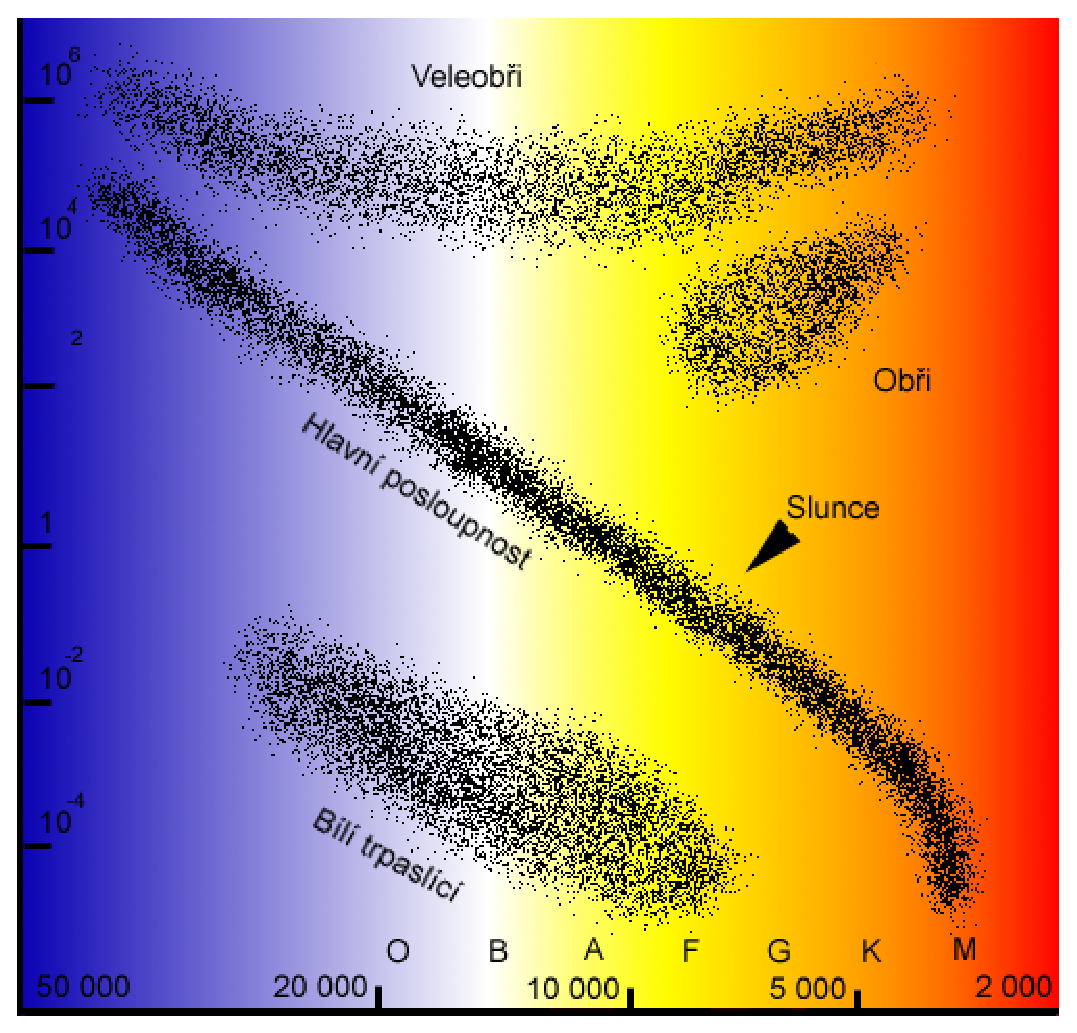
\includegraphics[width=80mm]{HR_diagram}
% where an .eps filename suffix will be assumed under latex, 
% and a .pdf suffix will be assumed for pdflatex; or what has been declared
% via \DeclareGraphicsExtensions.
\caption{HR diagram}
\label{HR_diagram}
\end{figure}
\paragraph{Co jsou to kuželosečky?}
Kuželosečka je rovinná křivka, která vznikne jako průnik roviny s pláštěm rotačního kuželu
(tzv. kuželová plocha), přičemž rovina neprochází jeho vrcholem. Obr. \ref{kuzelosecky}.
\begin{figure}[H]
\centering
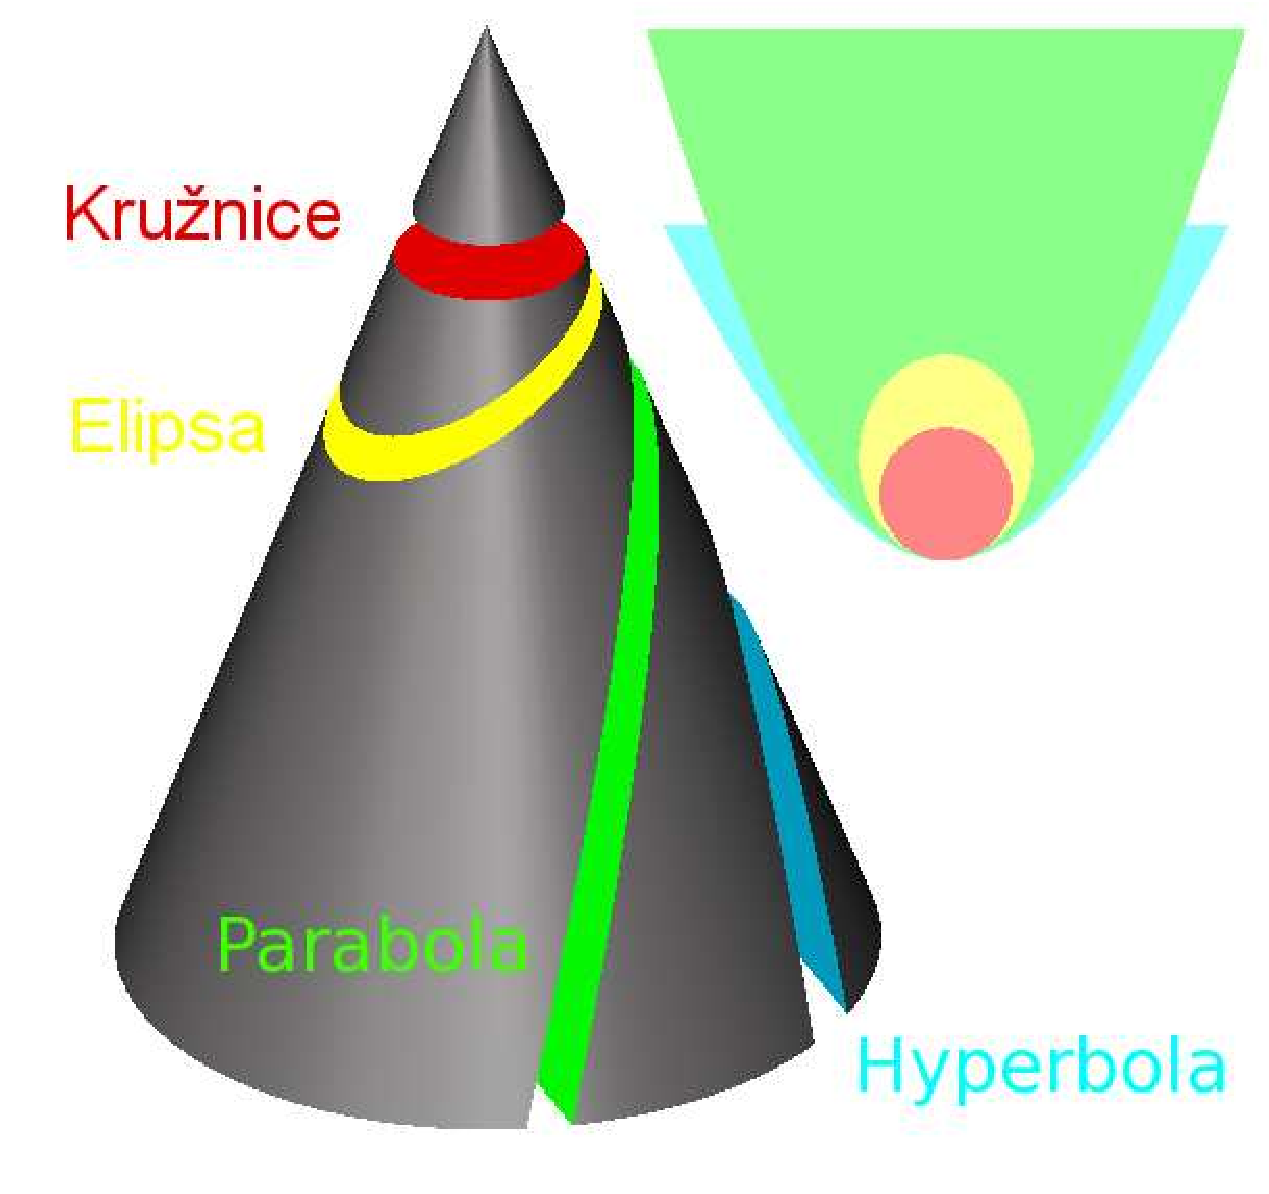
\includegraphics[width=80mm]{kuzelosecky}
% where an .eps filename suffix will be assumed under latex, 
% and a .pdf suffix will be assumed for pdflatex; or what has been declared
% via \DeclareGraphicsExtensions.
\caption{Kuželosečky}
\label{kuzelosecky}
\end{figure}
\paragraph{Po jakých trajektoriích se pohybují planety ve sluneční soustavě?}
\paragraph{Jakou numerickou výstřednost má elipsa?}
\paragraph{Jakou numerickou výstřednost má parabola?}
\paragraph{Co je první kosmická rychlost?}
\paragraph{Co je druhá kosmická rychlost?}
\paragraph{Co je třetí kosmická rychlost?}
\paragraph{Co je čtvrtá kosmická rychlost?}
\paragraph{Jakou rychlost musíme udělit projektilu, 
	aby se pohyboval po parabolické trajektorii?}
\paragraph{Jakým směrem musíme vystřelit projektil, 
	aby vzhledem ke Slunci měl co možná největší rychlost?}
\paragraph{Co je Eulerovo schéma (Eulerova metoda)?}
\paragraph{Mechanický princip relativity}
\paragraph{Einsteinovy postuláty STR}
\paragraph{Lorentzova transformace}
\paragraph{Dilatace času}
\paragraph{Kontrakce délek}
\paragraph{Časoprostorový interval}
\paragraph{Minkowského metrika}
\paragraph{Schwarzschildův poloměr}
\paragraph{Jak ovlivňuje gravitační pole chod času?}
\paragraph{Gravitační Dopplerův jev}
\paragraph{Fridmanova metrika}
\paragraph{Co vyjadřuje skalární křivost?}
\paragraph{Co vyjadřuje expanzní funkce?}
\paragraph{Kosmologický posuv}
\paragraph{Hubbleův zákon}
\paragraph{Hubbleův čas}
\paragraph{Jak starý je vesmír?}
\end{document}
